% ----------------------------------------------------
% Institute of Medical Informatics
% University of Luebeck
%
% Version 0.4
%
% ----------------------------------------------------

\documentclass[
%a4paper,
12pt,
headsepline,
bibliography=totoc,
twoside=semi,
fleqn
]{scrartcl}

\usepackage{pgf}
\usepackage{ucs}
\usepackage[latin1]{inputenc}
%\usepackage[pdftex]{graphicx}
\graphicspath{{./images/}}
\usepackage{color}
%\usepackage{german}
\usepackage{subfigure}
\usepackage{booktabs}
\usepackage{float}
\usepackage{wrapfig}

%% LAYOUT:

\renewcommand{\descfont}{\bfseries}
\renewcommand{\sectfont}{\bfseries}

\addtolength{\topmargin}{-1.5cm}
\addtolength{\textheight}{1.5cm}

\setkomafont{captionlabel}{\bfseries\footnotesize}
\setkomafont{caption}{\footnotesize}
\renewcommand{\headfont}{\bfseries}
\renewcommand{\figurename}{Fig.}
\renewcommand{\tablename}{Table}

\renewcommand*{\titlepagestyle}{empty}

\usepackage[automark]{scrlayer-scrpage}
\pagestyle{scrheadings}
\clearscrheadfoot
\rehead{\headmark} 
\lehead{\pagemark} 
\lohead{\headmark} 
\rohead{\pagemark}

\definecolor{Ocean}{cmyk}{1,0,0.2,0.78}
\definecolor{Grey}{cmyk}{0,0,0,0.6}

\usepackage{natbib}
\bibpunct{[}{]}{;}{a}{}{,}

\begin{document}

%==================================================
% TITLE PAGE
% -------------------------------------------------

\setlength{\headheight}{0pt}

\titlehead{
  \flushleft{
\includegraphics[width=0.7\textwidth]{Logo_Inst_MedInformatik_En_P309}}\\[-3.5ex]
  \centering
}

\subject{
\large{
  \vspace{0ex}
  \textnormal{Seminar}\\[1ex] 
  Medical Image Computing and e-Health\\[1ex]
  \textnormal{WS 2020/2021}\\[8ex]
}}

\title{
  \huge{\textcolor{Ocean}{Automatic Detection and Segmentation of Brain Tumor Using Random Forest Approach}}\\[5ex]
}

\author{
  \large{\textbf{Leonard Brenk}}\\
  \large{Matr.-Nr.: 697947, Computer Science}\\[5ex]
  \large{Supervisor}\\
  \large{Marja Fleitmann}\\[8ex]
}

\date{
  \large{Lübeck, \today}
  \pgfdeclareimage{university-slogan}{./images/Slogan_Uni_Luebeck_CMYK}
  \begin{pgfpicture}{0cm}{4cm}{14cm}{1.0cm}
    \pgfputat{\pgfpoint{10cm}{0cm}}{\pgfbox[left,bottom]{\pgfuseimage{university-slogan}}}
    \color {white}
%    \pgfputat{\pgfpoint{12.3cm}{0.4cm}}{\pgfbox[right,center]{  \insertshorttitle}}	
  \end{pgfpicture}
}


%============================CONTENT=========================

\maketitle
\newpage
\setcounter{page}{1}
\setlength{\headheight}{58pt}

%==================================================

\tableofcontents
\newpage

%==================================================
% TEXT
% -------------------------------------------------

\section{Motivation\label{sec:sec1}}
The detection and treatment of tumors is one of today's greatest challenges for mankind. Finding mutating cells and preventing them from spreading is an extraordinarily difficult task. Usually tumors occur nested in non-affected tissues which makes their discovery and treatment heavily challenging. The current state of technology operating in that field has complications filtering the negative cells out and segmenting the pure tumor completely. Due to the variety of anatomical structures and the way they can differ from person to person, even for a trained professional it takes a lot of time to detect and fully segment a tumor in MRI scans - even more if three-dimensional scans are used. Therefore not only are the needed financial and personal requirements greatly inefficient but also the outcome can be flawed and incomplete based on the know-how of the experts. Machine Learning ensembles provide a promising approach to face that issue on a global, revolutionary scale.\\

Seeing that finding the tumor in an early stage has the highest impact on and can facilitate and enhance the treatment the detection is the key to success. The paper written by \textcolor{red}{TODO AUTHOR} in 2016 captures an experiment regarding this topic. It carries out a Random Forest based machine learning technique using multispectral volumetric MRI volumes. Training an algorithm to reliably find and segment tumor cells on MRI scans can due to its practically limitless resources in time and memory possibly perform on a higher level than multiple experts. Therefore the data undergoes several steps of pre-processing in order to be suitable for the application in Binary Decision Trees. Furthermore, after the employment of Random Forests the data is post-processed and then analyzed. In order to illustrate the accuracy of a decision the authors introduced a Dice Score, thereby Binary Decision Trees can be compared and graded. The machine learning method used in this paper belongs to the supervised learning techniques which means that the outcome of data the machine is trained with is already known and can be used to adjust and optimize the inner parameters.\\

The paper presents initial outcomes and recommendations regarding a complex brain tumor detection and segmentation system and its future implementation in a clinical context.

\newpage
%--------------------------------------------------

\section{Introduction BDT \& RDF\label{sec:sec2}}
In this section the essential basics regarding Binary Decision Trees and Random Forest and their implementation are being explained an discussed.

  \subsection{Binary Decision Trees(BDT)\label{sec:sec2-1}}

    \subsubsection{General\label{sec:sec2-1-1}}
      A Binary Decision Tree (BDT) is trained and employed in order to make a decision based on a data vector. It consists of multiple levels of two-way decisions until it reaches a leaf node at the end classifying the vector into a certain class. A BDT can be used to either deploy data into classes or predict values in the future using regression. However, this paper will concentrate on the ability to assign a label to a vector. 

      \begin{figure}[H]
        \centering 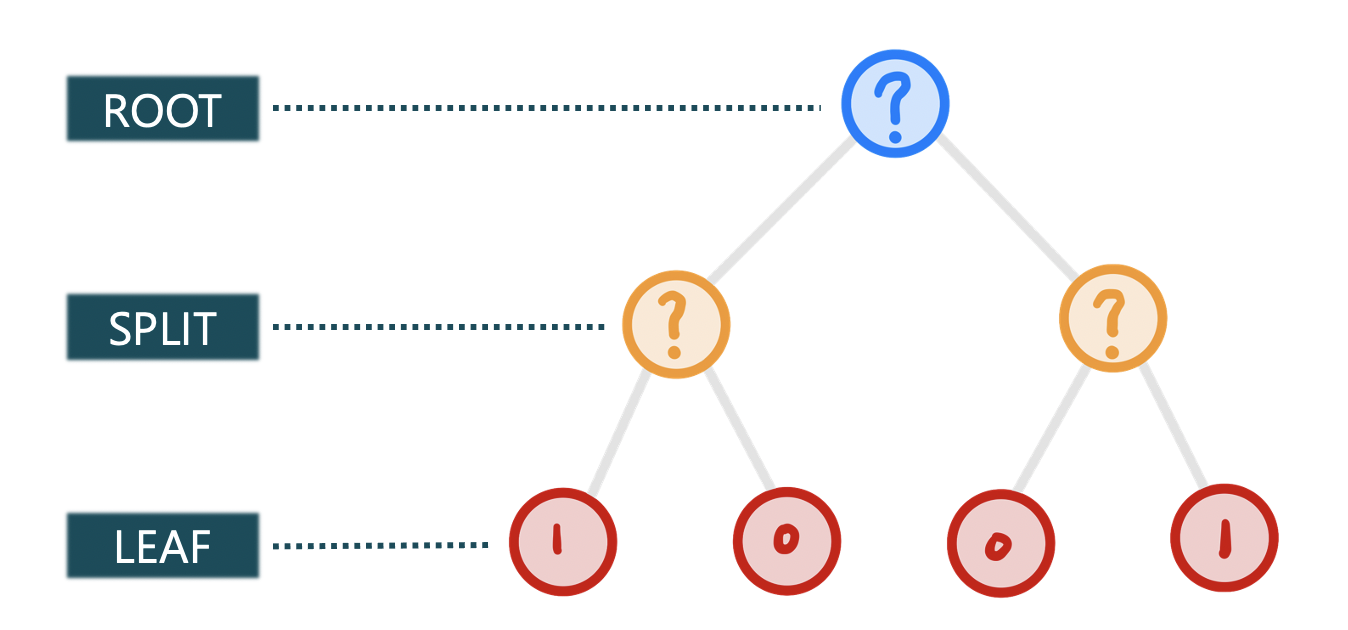
\includegraphics[scale=0.55]{BDT1.png}\label{fig:fig1}
        \caption{The Structure of a BDT. Usually there are multiple levels of split nodes.}
      \end{figure}

      The root node is the starting point of a BDT. In order for a BDT to reach a decision it goes through several inner decision nodes which divide the data into two subgroups and forwards them to the next node. At each split node the data is divided again as long as the decisions within the data subset are distinguishable. If the decisions are unilateral, a leaf node is created. Such leaf nodes are then attributed to a class, also called a label. Thereby an inserted data vector can be classified into classes. 

    \subsubsection{Building a BDT\label{sec:sec2-1-2}}
      A BDT can, amongst other options, be build from a table which contains multiple attributes and a column for the individual decision of that data row. When building a BDT a cycle is implemented recursively. The data shall be divided into two subgroups at a time. Then each subgroup is again divided into two subgroups. In the end there are as many subgroups as it takes to classify every single data vector correctly. The cycle starts with a given data set. For the first split an attribute needs to be picked which the data shall be split with. Having decided upon that attribute, a threshold is set to decided wether a vector is forwarded to the left or right child node - depending on whether its value is higher or smaller than the threshold. Using the threshold the complete data set can then be divided into two subgroups. Now each subgroup is considered individually and the cycle begins again. The process ends when the decisions of a subgroup are all identical. Then the leaf node is created labeled with that decision.  

      \begin{figure}[H]
        \centering 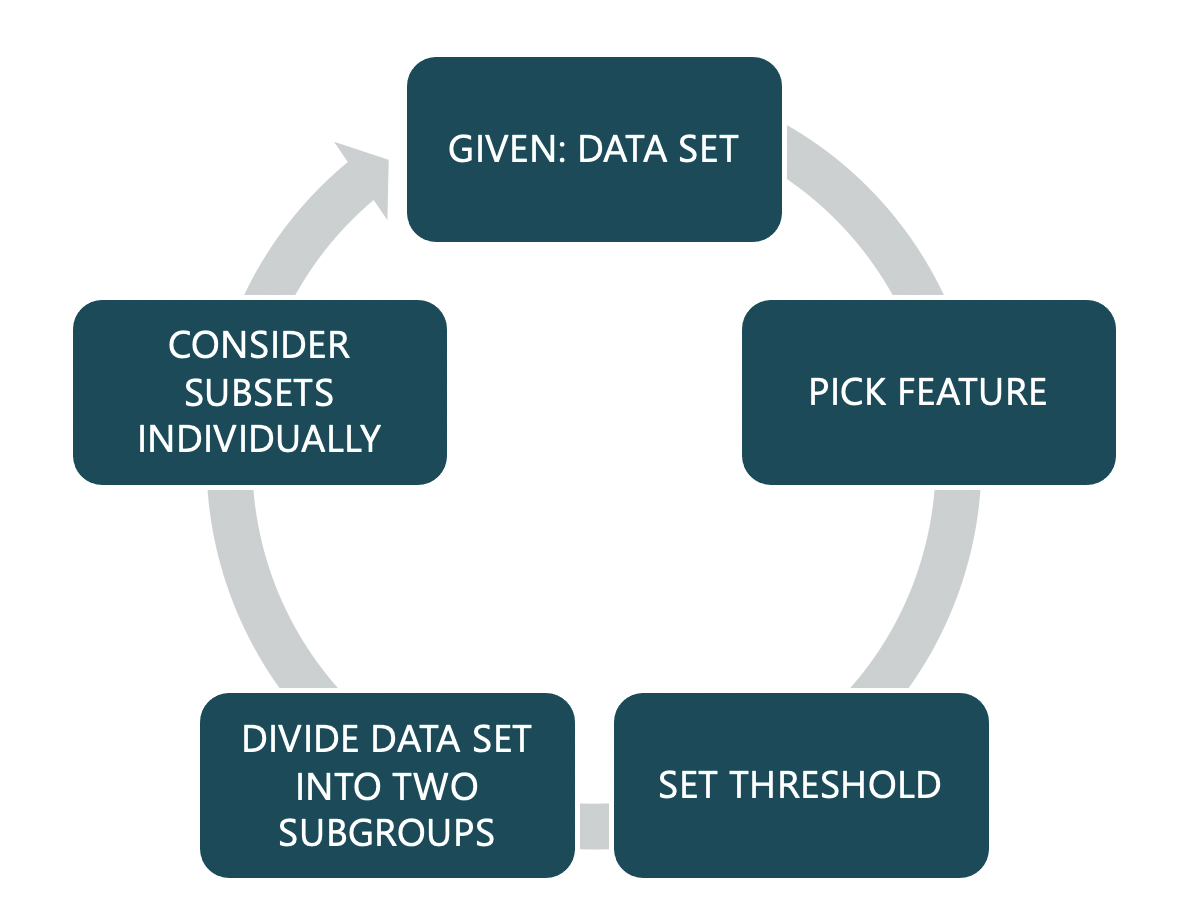
\includegraphics[scale=0.55]{BDT2.png}\label{fig:fig2}
        \caption{The process of buidling a BDT.}
      \end{figure}


      The decision for a specific feature while building a BDT can influence the outcome greatly since the generated subgroups will be completely different. That is why there is need for a way to assess the most efficient way of splitting the data. For that the information entropy and information gain are used. The entropy describes the level of information of a variable (\ref{fig:fig3}). The information gain compares two entropies and calculates the difference(\ref{fig:fig4}). The idea is to test every attribute as a possible option for a split node and calculate which attribute would yield the highest gain in information after the split. 

      \begin{figure}[h]
        \center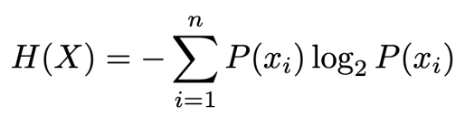
\includegraphics[scale=0.55]{BDT3.png}\label{fig:fig3}\caption{Entropy}
        \center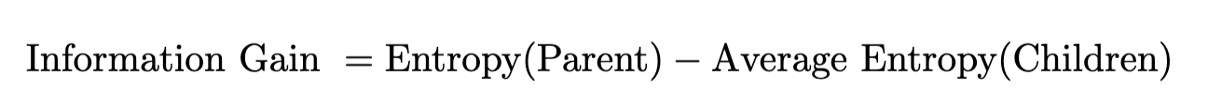
\includegraphics[scale=0.55]{BDT4.png}\label{fig:fig4}\caption{Information Gain}
      \end{figure}

    \subsubsection{Example BDT\label{sec:sec2-1-3}}
      Given a table of sample data: \\
      
      \begin{center}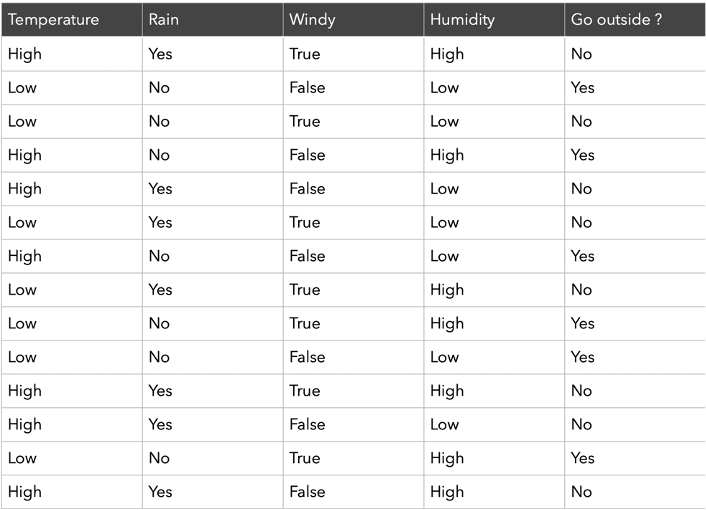
\includegraphics[scale=0.7]{BDT5.png}\label{fig:fig5}\end{center}
      
      In order to decide which attribute to pick for the root node, the information gain must be calculated for all of them (Temperature, Rain, Windy and Humidity). For example Splitting with Temperature would look like this: \\

      First we need to calculate the entropy of the complete table. 

      \begin{center}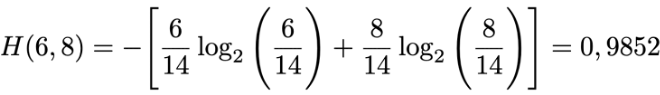
\includegraphics[scale=0.7]{BDT8.png}\label{fig:fig8}\end{center}

      If we were to split at Temperature the table would be divided into two groups, one with high temperature and one with low temperature. Now the entropy for both of these subgroups needs to be calculated individually. The information gain for Temperature is the difference resulting from the complete entropy minus the average entropy of the new generated subgroups. In this case the information gain is $0,01615$. 

      \begin{center}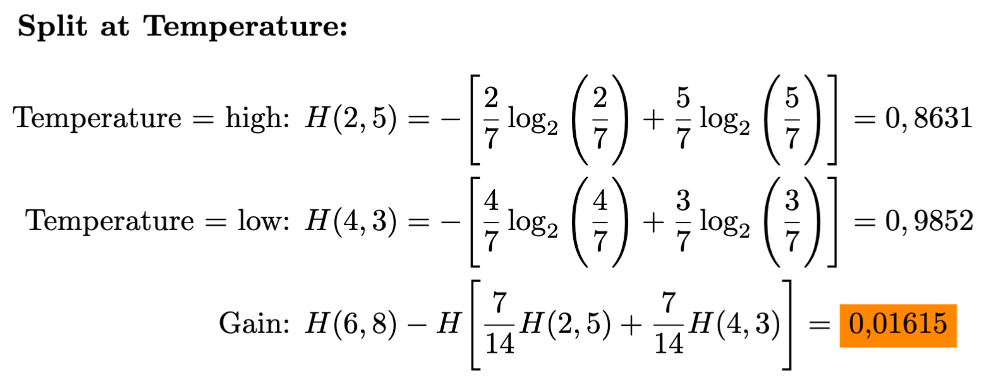
\includegraphics[scale=0.7]{BDT7.png}\label{fig:fig7}\end{center}

      Since the information gain is the value that needs to be maximized, the information gain is calculated for the remaining attributes as well. For the root node the attribute is selected that yields the highest information gain. In this case: Rain. 

      \begin{center}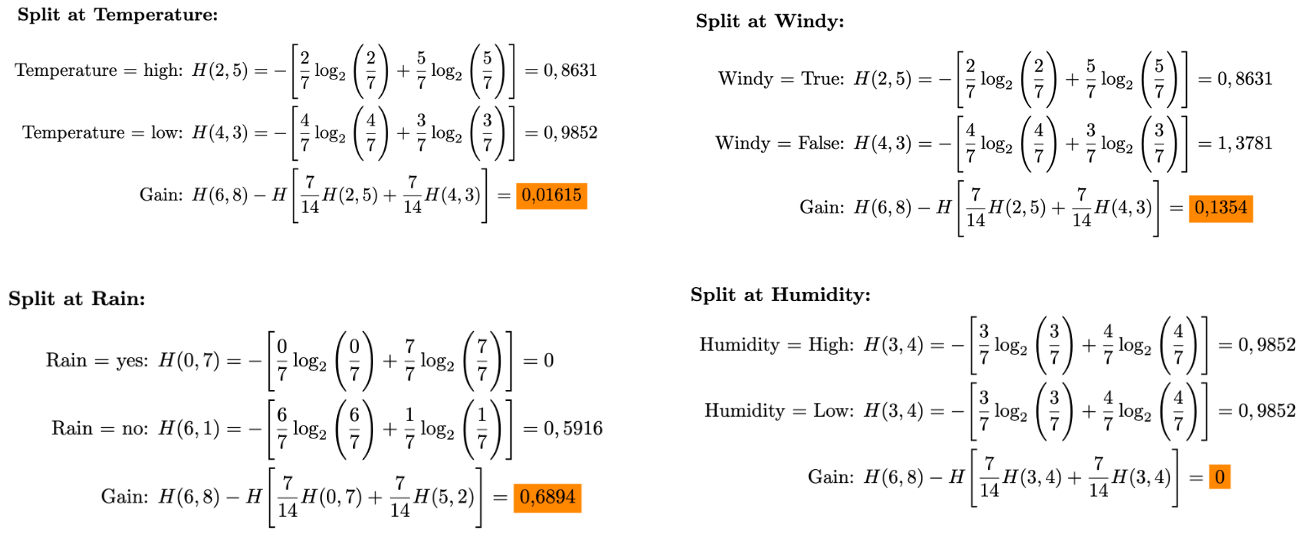
\includegraphics[scale=0.7]{BDT9.png}\label{fig:fig9}\end{center}

      Having split the data with rain, two subgroups are created \ref{fig:fig10}. Selecting the attribute for the next split node for a subgroup proceeds exactly like with the root node, only with a smaller set of data. The final tree will then look like this: 

      \begin{figure}[H]
        \centering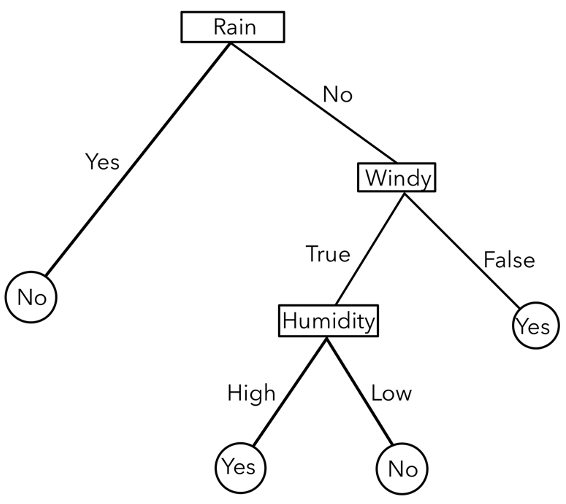
\includegraphics[scale=0.7]{BDT11.png}\label{fig:fig11}
        \caption{The final BDT.}
        \end{figure}
      

      \begin{figure}[H]
      \centering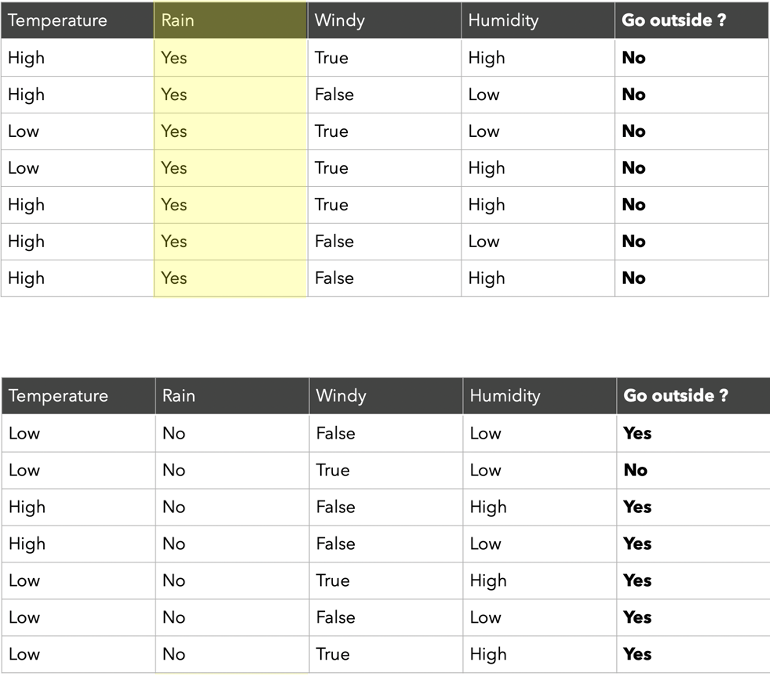
\includegraphics[scale=0.7]{BDT10.png}\label{fig:fig10}
      \caption{The two generated subgroups when splitting with Rain at the root node.}
      \end{figure}
  
    \subsubsection{Testing a BDT\label{sec:sec2-1-4}}
      After building a BDT it has to be ensured that it is working correctly and classifies properly. Therefore not all data is used for building the tree but a part is saved for testing purposes. Now that the BDT is build we can pick samples of the test data and insert it into the BDT. As this is a supervised learning ensemble the result is already known and can thereby be compared with the yielded outcome of the tree. If it is correct, the tree is working fine. The accuracy characterizing Dice Score is based on testing cases and describes their outcome in a numerical, understandable way. 

    \subsubsection{Pro and Cons of BDT\label{sec:sec2-1-5}}
      A BDT can be used to classify and label data vectors which can be helpful for a lot of problems. As is it not limited to categorical values for classification but can also work with numerical values, a BDT is also able to predict future values through regression curves. Furthermore the technique and structure of a BDT and its decision finding process is intuitive and visualizable. Additionally the data used only requires little data pre-processing \textcolor{red}{TODO WHY}.

      The problem with BDTs is that small changes in data can heavily affect the outcome of the decision. If the tree internalizes every detail of the training data it can overfit. That means that the BDT doesn't reflect the general input data but has adapted to the training data. For instance: If an algorithm was given scans of tumors that are compared to all other existing tumor scans rather dark than the BDT will set this as the general intensity of a tumor scan. Thereby brighter parts of tumors scans that the BDT has not seen yet will not be classified as tumor. In order to face that issue Random Forests have been intoruced.   



  \subsection{Random Forest(RDF)\label{sec:sec2-2}}

\section{Application\label{sec:sec3}}

  \subsection{Goal of the Paper\label{sec:sec3-1}}
  \subsection{Data \& Pre-Processing\label{sec:sec3-2}}
  \subsection{Training and Testing\label{sec:sec3-3}}
  \subsection{Post-Processing\label{sec:sec3-4}}

\section{Results\label{sec:sec4}}

\section{Conclusion\label{sec:sec5}}

\section{Sources \& Appendix\label{sec.sec5}}

%--------------------------------------------------
% Example of a figure with subfigures
%--------------------------------------------------

\newpage
\begin{figure}[p]
\centering
\subfigure[]{
  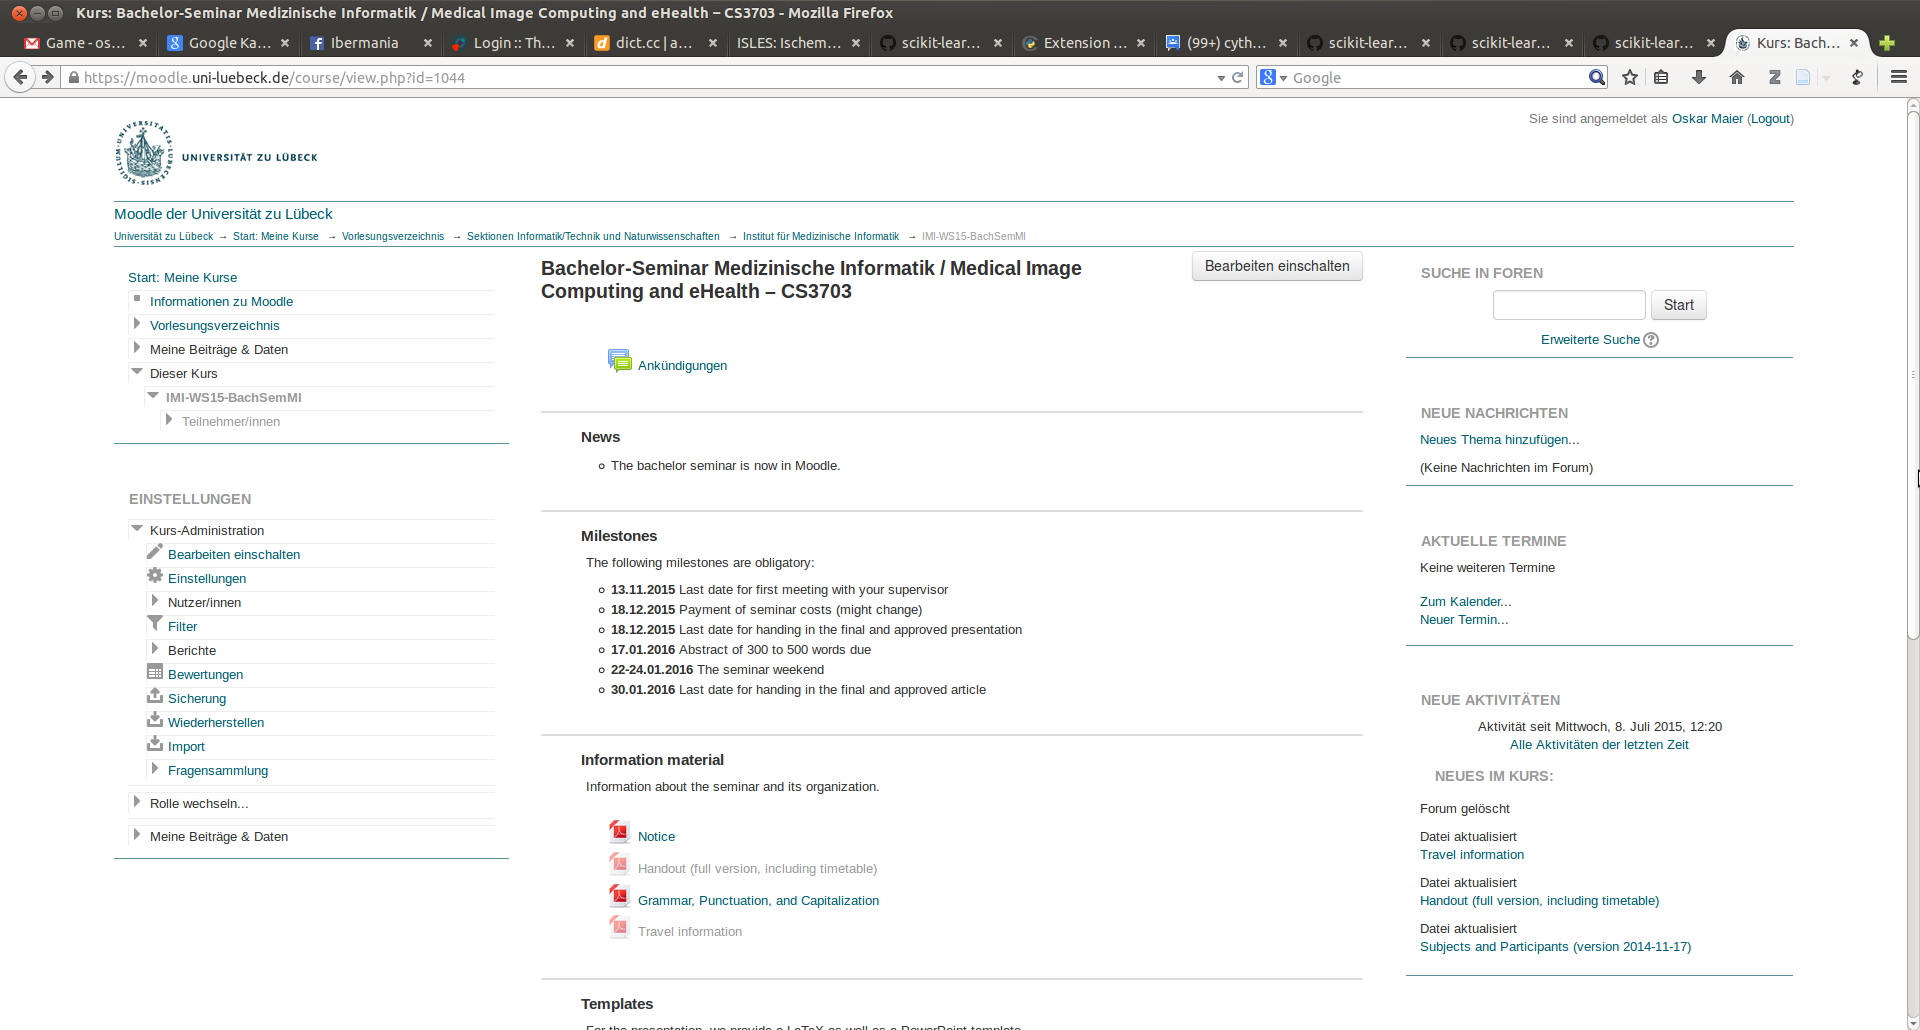
\includegraphics[width=\textwidth]{Moodle4}
  \label{fig:subfig1}
}
\subfigure[]{
  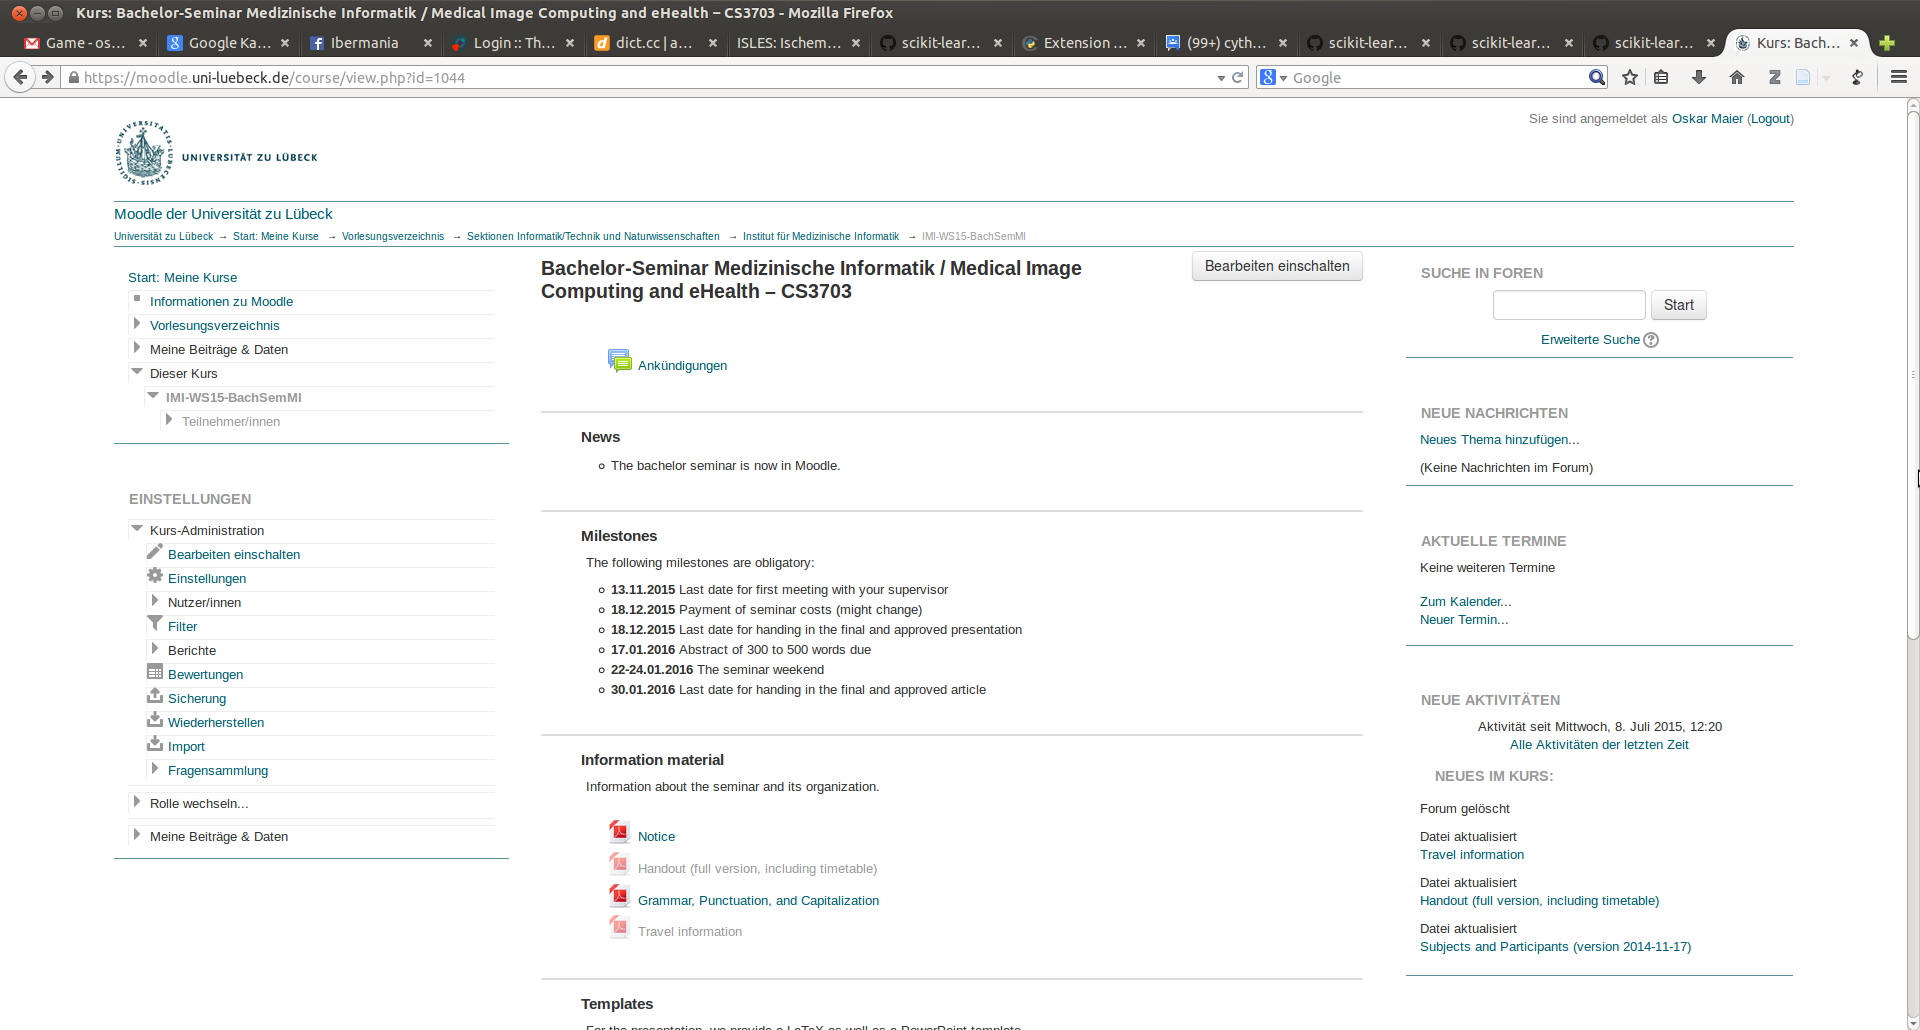
\includegraphics[width=\textwidth]{Moodle4}
  \label{fig:subfig2}
}
\caption{Two times (\subref{fig:subfig1} and \subref{fig:subfig2}) the Moodle page for this seminar.}
\label{fig:subfigureExample}
\end{figure}

%--------------------------------------------------
% Example of a table
%--------------------------------------------------


\begin{table}[t]
    \footnotesize
    \caption{\label{tab:table1} Topics of the presentations \textbf{two years ago}.}
    \vspace{1ex}
    \centering 
    \begin{tabular}{p{2.5cm}p{8.7cm}p{2.8cm}}
        \toprule
        \textbf{Speaker} & \textbf{Topic [Literature]} & \textbf{Supervisor} \\
        \midrule
        J. Niemeijer & Hough transforms & M. Wilms \\
        D. Labitzke & Optimal Surface Segmentation in Volumetric Images -- A Graph-Theoretic Approach (cf. \citep{Li_TPAMI_2006}) & M. Wilms \\
        A. Bostelmann & Graph Cuts for image segmentation
        & O. Maier \\
        D. Conrad & Texture descriptors and their application to medical images & O. Maier
        \\
        E. Franke & Image Segmentation Using Deformable Models: Parametric Deformable
        Models & J. Kr�ger \\
        N. Broecker & Image Segmentation Using Deformable Models:Geometric Deformable
        Models & J. Kr�ger \\
        L. Pankert & Visualization in Medicine: Volume Rendering with ray-casting
        & J. Ehrhardt \\
        T. Langer & Visualization in Medicine: Surface Rendering using the Marching Cubes
        Algorithm & J. Ehrhardt \\
        M. Caspe & Volumetric Ultrasound Stitching & D. Fortmeier \\
        H. T�nnies & Surface-based Palpation Haptics & D. Fortmeier \\
        \midrule
        P. Kling & A Content Model for the ICD-11 Revision & J. Ingenerf \\
        S. Heusel & MeSHy: Mining unanticipated PubMed information using frequencies of
        occurrences and concurrences of MeSH terms & J. Ingenerf \\
        K. Soika & What is bioinformatics? An introduction and overview & B. Andersen \\
        M. Licht & How (not) to protect genomic data privacy in a distributed network: using trail
        re-identification to evaluate and design anonymity protection systems & J. Ingenerf \\
        J. Fleckner & Adverse events in medicine: Easy to count, complicated to understand, and
        complex to prevent & A.-K. Kock \\
        A. Wiegmann & An automated technique for identifying associations between medications,
        laboratory results and problems & A.-K. Kock \\
        J.-H. Mathes & Organization of Heterogeneous Scientific Data Using the EAV/CR
        Representation & B. Andersen\\
        F. Simon & Structured Reporting: Patient Care Enhancement or Productivity Nightmare? & A.-K. Kock\\
        \bottomrule
    \end{tabular}
    \vspace{2ex}
\end{table}


%==================================================
\newpage
%\bibliographystyle{plain}
\bibliographystyle{elsarticle-harv}
\footnotesize\bibliography{bib}


\end{document}
